\documentclass[conference]{IEEEtran}
\IEEEoverridecommandlockouts

\usepackage{cite}
\usepackage{amsmath,amssymb,amsfonts}
\usepackage{graphicx}
\usepackage{textcomp}
\usepackage{xcolor}
\usepackage{booktabs}
\usepackage{url}
\usepackage{hyperref}
\hypersetup{colorlinks=true, linkcolor=blue, citecolor=blue, urlcolor=blue}

\graphicspath{{../figures/}}

\begin{document}

\title{Improving Tip-of-the-Tongue Retrieval with\\Transformer-Based Reranking\\
{\large Phase 2: Experiment Tracking, BM25 Baseline, and Preliminary Reranker Results}}

\author{\IEEEauthorblockN{\.Ilayda Erg\"ur}
\IEEEauthorblockA{Department of Multimedia Informatics\\
Middle East Technical University\\
Ankara, Turkey\\
ilayda.ergur@metu.edu.tr}}

\maketitle

\begin{abstract}
This report presents the second phase of an ongoing investigation into
transformer-based reranking for Tip-of-the-Tongue (ToT) retrieval.
Building on the exploratory analysis of Phase~1, we introduce a fully
reproducible two-stage retrieval pipeline:
a BM25 first-stage retriever tuned via a Weights \& Biases parameter sweep,
followed by a cross-encoder reranker (\texttt{ms-marco-MiniLM-L-6-v2}).
All experiments are conducted on the TREC-ToT 2025/dev1 split (142 queries,
same 2024 corpus).
BM25 achieves RR@10~=~0.0751 and nDCG@10~=~0.0812.
The cross-encoder reranker scores RR@10~=~0.0463 and nDCG@10~=~0.0635,
falling below the BM25 baseline; a Wilcoxon signed-rank test confirms
this difference is not statistically significant ($p = 0.1023$).
A key finding is that all 142 queries have zero Jaccard keyword overlap
with their top-ranked BM25 result, confirming the purely semantic nature
of ToT queries and motivating stronger semantic models for future work.
\end{abstract}

\begin{IEEEkeywords}
information retrieval, tip-of-the-tongue, BM25, cross-encoder reranking,
dense retrieval, bi-encoder, TREC, Weights \& Biases, Wilcoxon test
\end{IEEEkeywords}

% ══════════════════════════════════════════════════════════════════════════════
\section{Introduction}
% ══════════════════════════════════════════════════════════════════════════════

Phase~1 of this project established that the TREC Tip-of-the-Tongue 2024
dataset poses exceptional challenges for lexical retrieval systems: queries
average 238 words, documents average over 6{,}700 words, and the vocabulary
gap between descriptive queries and formal Wikipedia text is large.
These observations motivated a two-stage architecture in which BM25 produces
an initial candidate set that a semantic model then reranks.

Phase~2 realises this architecture end-to-end.
An important observation from the TREC-ToT task design is that
\emph{all} queries are by construction long and narrative, and
\emph{all} have near-zero lexical overlap with relevant documents.
Treating query length and keyword overlap as independent subgroup variables
would therefore collapse into the same experiment.
We instead define three distinct research questions that each isolate a
different variable:

\begin{itemize}
  \item \textbf{RQ1:} Does cross-encoder reranking significantly improve
        retrieval effectiveness over a BM25 baseline for Tip-of-the-Tongue
        queries (Wilcoxon signed-rank test, $\alpha=0.05$)?
  \item \textbf{RQ2:} Is the reranker's gain modulated by query length
        (within the ToT population), given that longer queries suffer greater
        truncation under the 512-token cross-encoder limit?
  \item \textbf{RQ3 (Phase 3):} Does replacing the BM25 first stage with
        dense bi-encoder retrieval improve effectiveness on a task where
        lexical matching is structurally insufficient?
\end{itemize}

RQ3 is scoped to Phase~3; this report establishes the BM25 and cross-encoder
baselines that RQ3 will be measured against.

% ══════════════════════════════════════════════════════════════════════════════
\section{Dataset and Evaluation Setup}
\label{sec:dataset}
% ══════════════════════════════════════════════════════════════════════════════

\subsection{Corpus and Queries}

The TREC Tip-of-the-Tongue 2024 corpus contains 3{,}185{,}450 English Wikipedia
documents.
We use the \texttt{trec-tot/2025/dev1} query set (the same corpus), which
provides 142 queries with publicly available relevance judgements (qrels).
The 2024 test split's qrels are not publicly released; the 2025/dev1 split
was therefore used as the evaluation set throughout all experiments.
All data is accessed via the \texttt{ir\_datasets} library~\cite{irdatasets}.

\subsection{Metrics}

We report three standard metrics:
\begin{itemize}
  \item \textbf{RR@10} (Reciprocal Rank at 10, mean = MRR@10): captures
        whether the top-10 results contain at least one relevant document
        and how highly it is ranked.
  \item \textbf{nDCG@10}: measures the quality of the full top-10 ranking.
  \item \textbf{R@100}: recall of all relevant documents in the top-100,
        which reflects first-stage retrieval coverage.
\end{itemize}

All metrics are computed with PyTerrier's \texttt{pt.Experiment}
backed by \texttt{ir\_measures}~\cite{irm}.

% ══════════════════════════════════════════════════════════════════════════════
\section{Experiment Tracking with Weights \& Biases}
\label{sec:wandb}
% ══════════════════════════════════════════════════════════════════════════════

All experiments are logged to the public Weights \& Biases
project \texttt{is584-tot-retrieval}\footnote{\url{https://wandb.ai/ilaydaergur/is584-tot-retrieval}}.
WANDB tracks hyperparameters, metrics, and run metadata, enabling full
reproducibility and comparison across runs.

\begin{figure}[t]
  \centering
  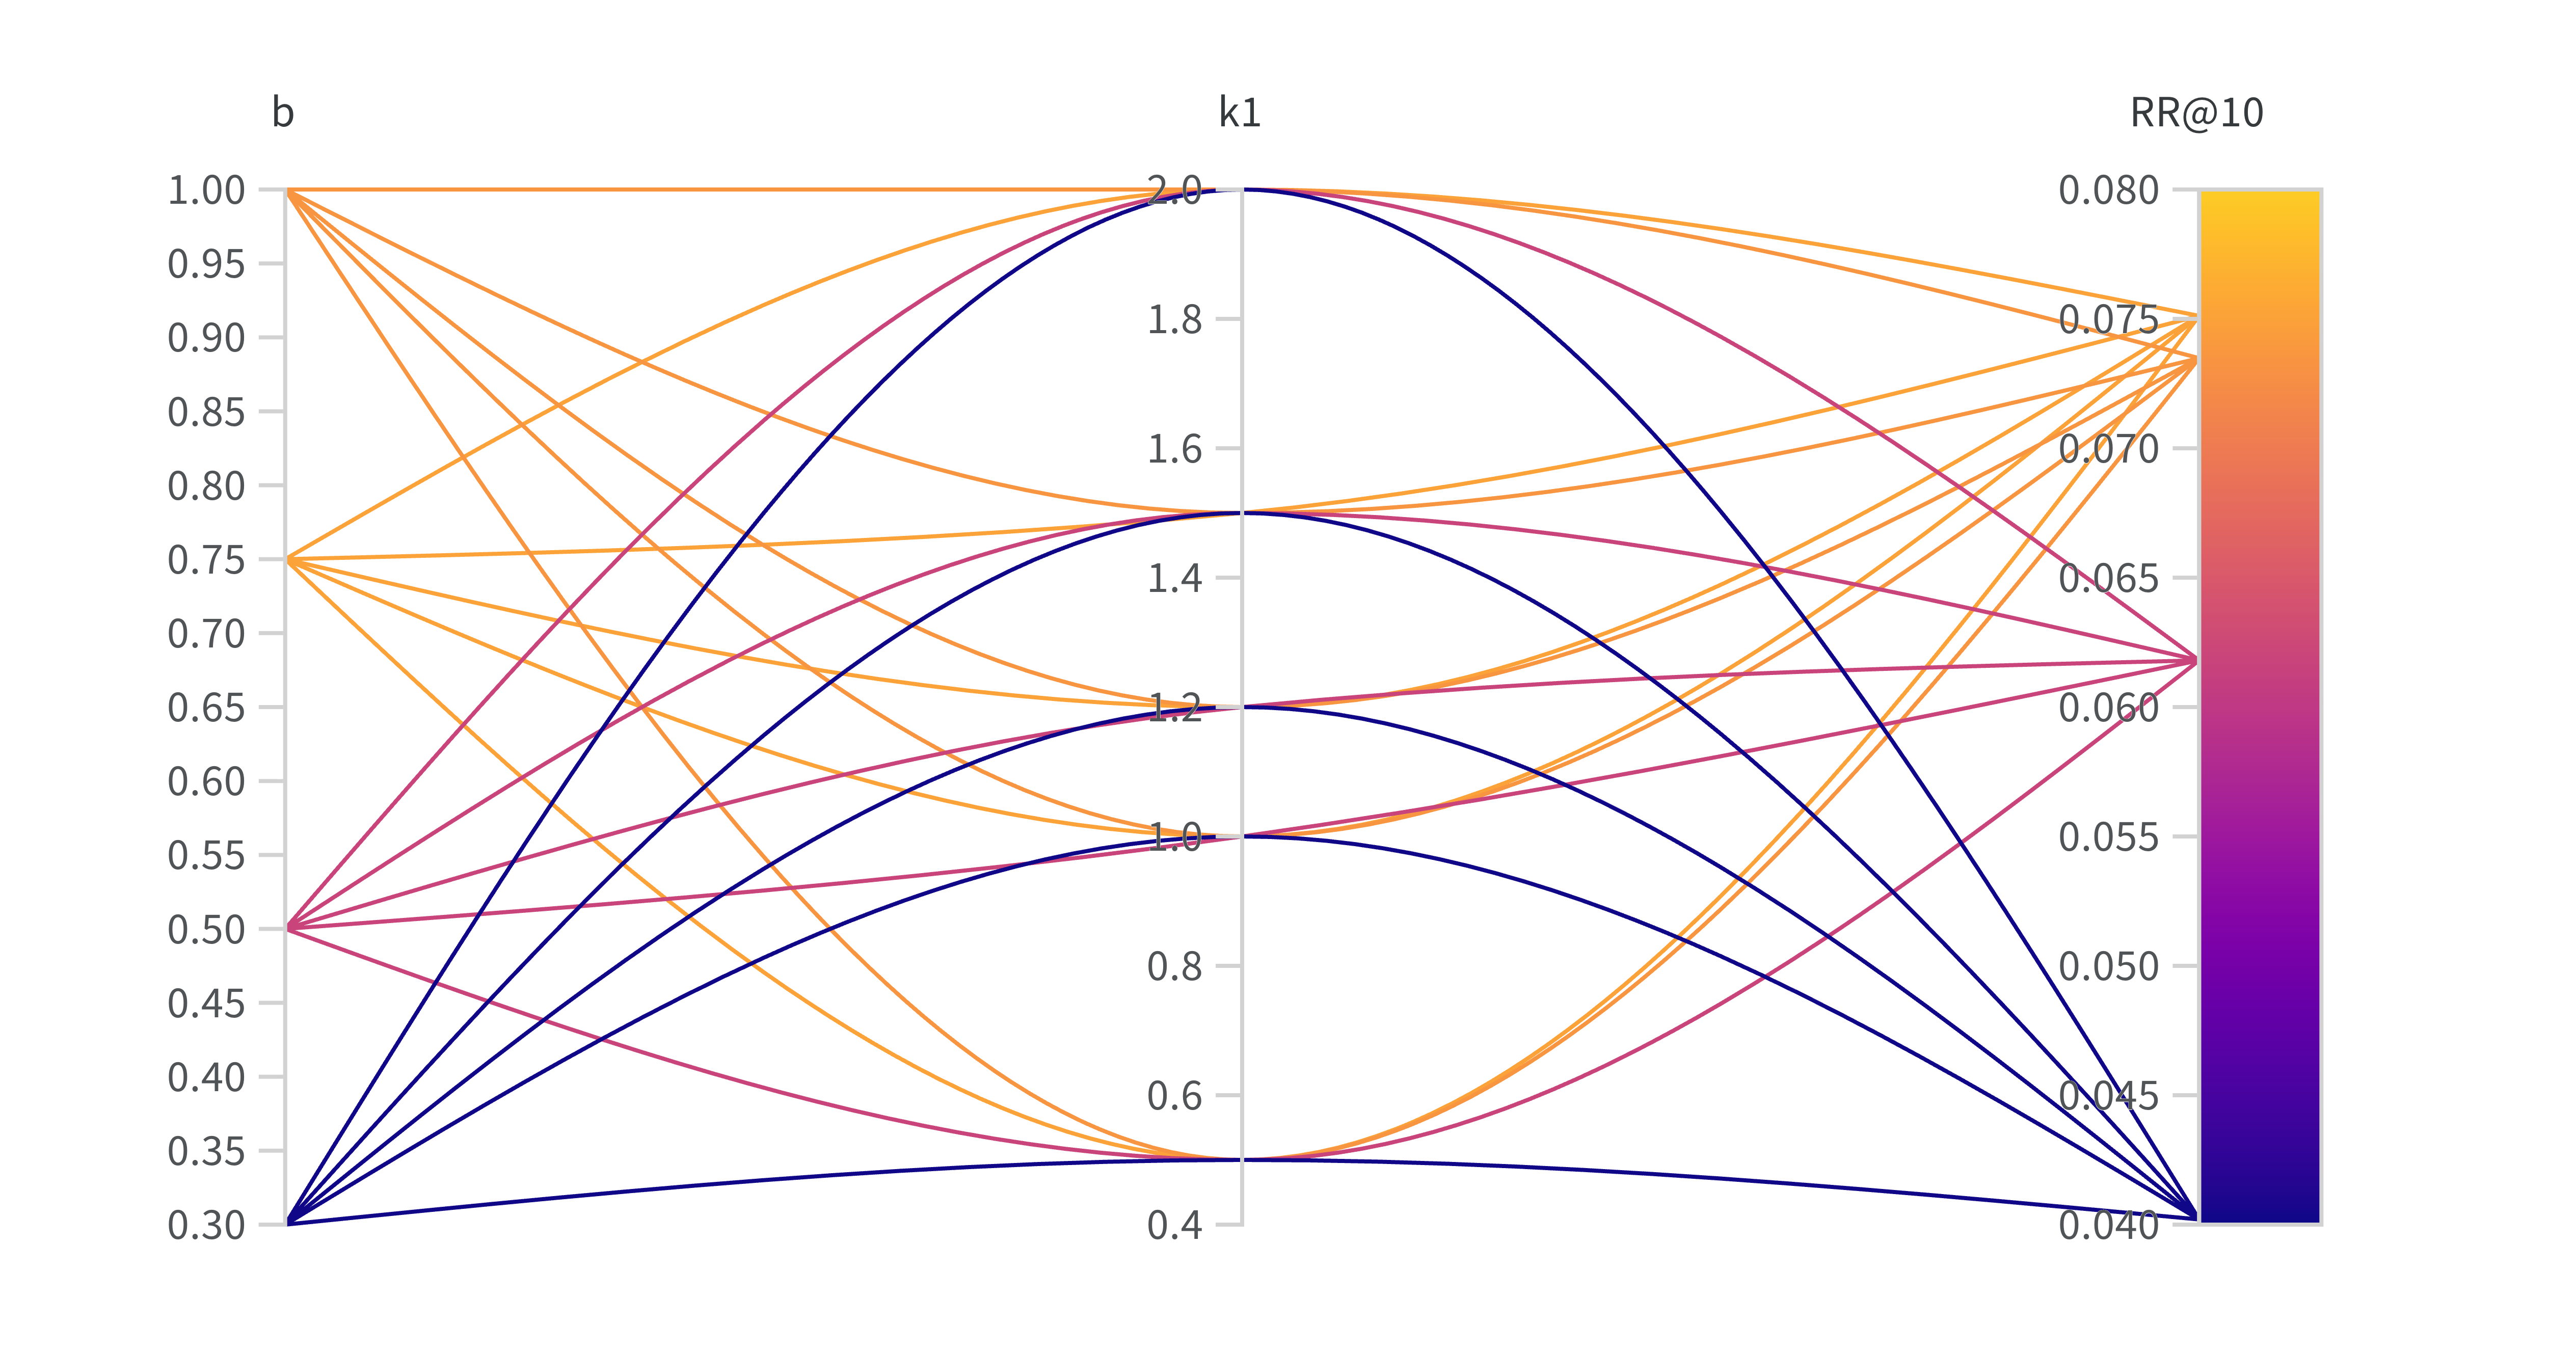
\includegraphics[width=\columnwidth]{wandb_sweep.png}
  \caption{WANDB parallel-coordinates plot of the BM25 grid sweep (20 runs).
           Each line represents one ($k_1$, $b$) configuration; colour encodes
           RR@10 (yellow $\approx$ 0.080 = best, dark blue $\approx$ 0.040 = worst).
           Runs with $k_1 \in [1.2, 1.5]$ and $b = 0.75$ consistently achieve
           the highest scores.}
  \label{fig:wandb}
\end{figure}

\subsection{BM25 Parameter Sweep}

A grid sweep was run over BM25 hyperparameters:
$k_1 \in \{0.5, 1.0, 1.2, 1.5, 2.0\}$ and
$b \in \{0.3, 0.5, 0.75, 1.0\}$,
totalling 20 runs.
Figure~\ref{fig:wandb} shows the parallel-coordinates visualisation from WANDB;
Table~\ref{tab:sweep} lists the top-5 configurations by RR@10.
The best configuration found was $k_1=1.2$, $b=0.75$, which is also the
commonly recommended BM25 default and was used for all subsequent experiments.

\begin{table}[t]
\caption{Top-5 BM25 Configurations from the WANDB Sweep}
\label{tab:sweep}
\centering
\begin{tabular}{cccc}
\toprule
$k_1$ & $b$ & RR@10 & nDCG@10 \\
\midrule
1.2 & 0.75 & \textbf{0.0751} & \textbf{0.0812} \\
1.0 & 0.75 & 0.0737 & 0.0799 \\
1.5 & 0.75 & 0.0730 & 0.0805 \\
1.2 & 0.50 & 0.0718 & 0.0790 \\
2.0 & 0.75 & 0.0714 & 0.0798 \\
\bottomrule
\end{tabular}
\end{table}

% ══════════════════════════════════════════════════════════════════════════════
\section{BM25 Baseline}
\label{sec:bm25}
% ══════════════════════════════════════════════════════════════════════════════

\subsection{Implementation}

The BM25 index was built with PyTerrier's \texttt{IterDictIndexer}
over the full 3.18M-document corpus.
Two fields are indexed (\texttt{text}, \texttt{title}); a 2{,}000-character
text snippet is stored as document metadata so the reranker can score
(query, document) pairs without a second corpus pass.
Retrieval returns up to 100 candidates per query.

\subsection{Results}

Table~\ref{tab:aggregate} reports aggregate metrics for the BM25 baseline.
With R@100~=~0.218, approximately 22\% of relevant documents appear in the
top-100 candidates, providing the reranker's ceiling.
The RR@10 of 0.075 reflects the inherent difficulty of the task:
most queries receive no relevant result in the top 10.

% ══════════════════════════════════════════════════════════════════════════════
\section{Preliminary Reranker Results}
\label{sec:reranker}
% ══════════════════════════════════════════════════════════════════════════════

\subsection{Model and Implementation}

The cross-encoder model \texttt{cross-encoder/ms-marco-MiniLM-L-6-v2}
was used to score all (query, document) pairs in the top-100 BM25 candidates.
This model was chosen for efficiency (6-layer MiniLM) while retaining strong
reranking capability from MS-MARCO training.

ToT queries average 238 words, far exceeding the 512-token limit of the
cross-encoder when combined with a document snippet.
To allocate sufficient token budget to the document, each query is
truncated to its first 100 words before scoring.
Documents use the 2{,}000-character snippet stored at index time.
Inference was run in batches of 32 pairs on CPU/MPS.

\subsection{Aggregate Results}

\begin{table}[t]
\caption{Aggregate Retrieval Metrics on trec-tot/2025/dev1 (n=142 queries)}
\label{tab:aggregate}
\centering
\begin{tabular}{lccc}
\toprule
System & RR@10 & nDCG@10 & R@100 \\
\midrule
BM25 ($k_1$=1.2, $b$=0.75) & 0.0751 & 0.0812 & 0.2183 \\
CrossEncoder reranker       & 0.0463 & 0.0635 & 0.2183 \\
\midrule
$\Delta$ (Reranker $-$ BM25) & $-$0.0288 & $-$0.0177 & 0.0000 \\
\bottomrule
\end{tabular}
\end{table}

Figure~\ref{fig:aggregate} visualises the metric comparison.
The reranker does not improve over BM25 on any metric in aggregate;
R@100 is identical because both systems operate on the same first-stage
candidate set.

\begin{figure}[t]
  \centering
  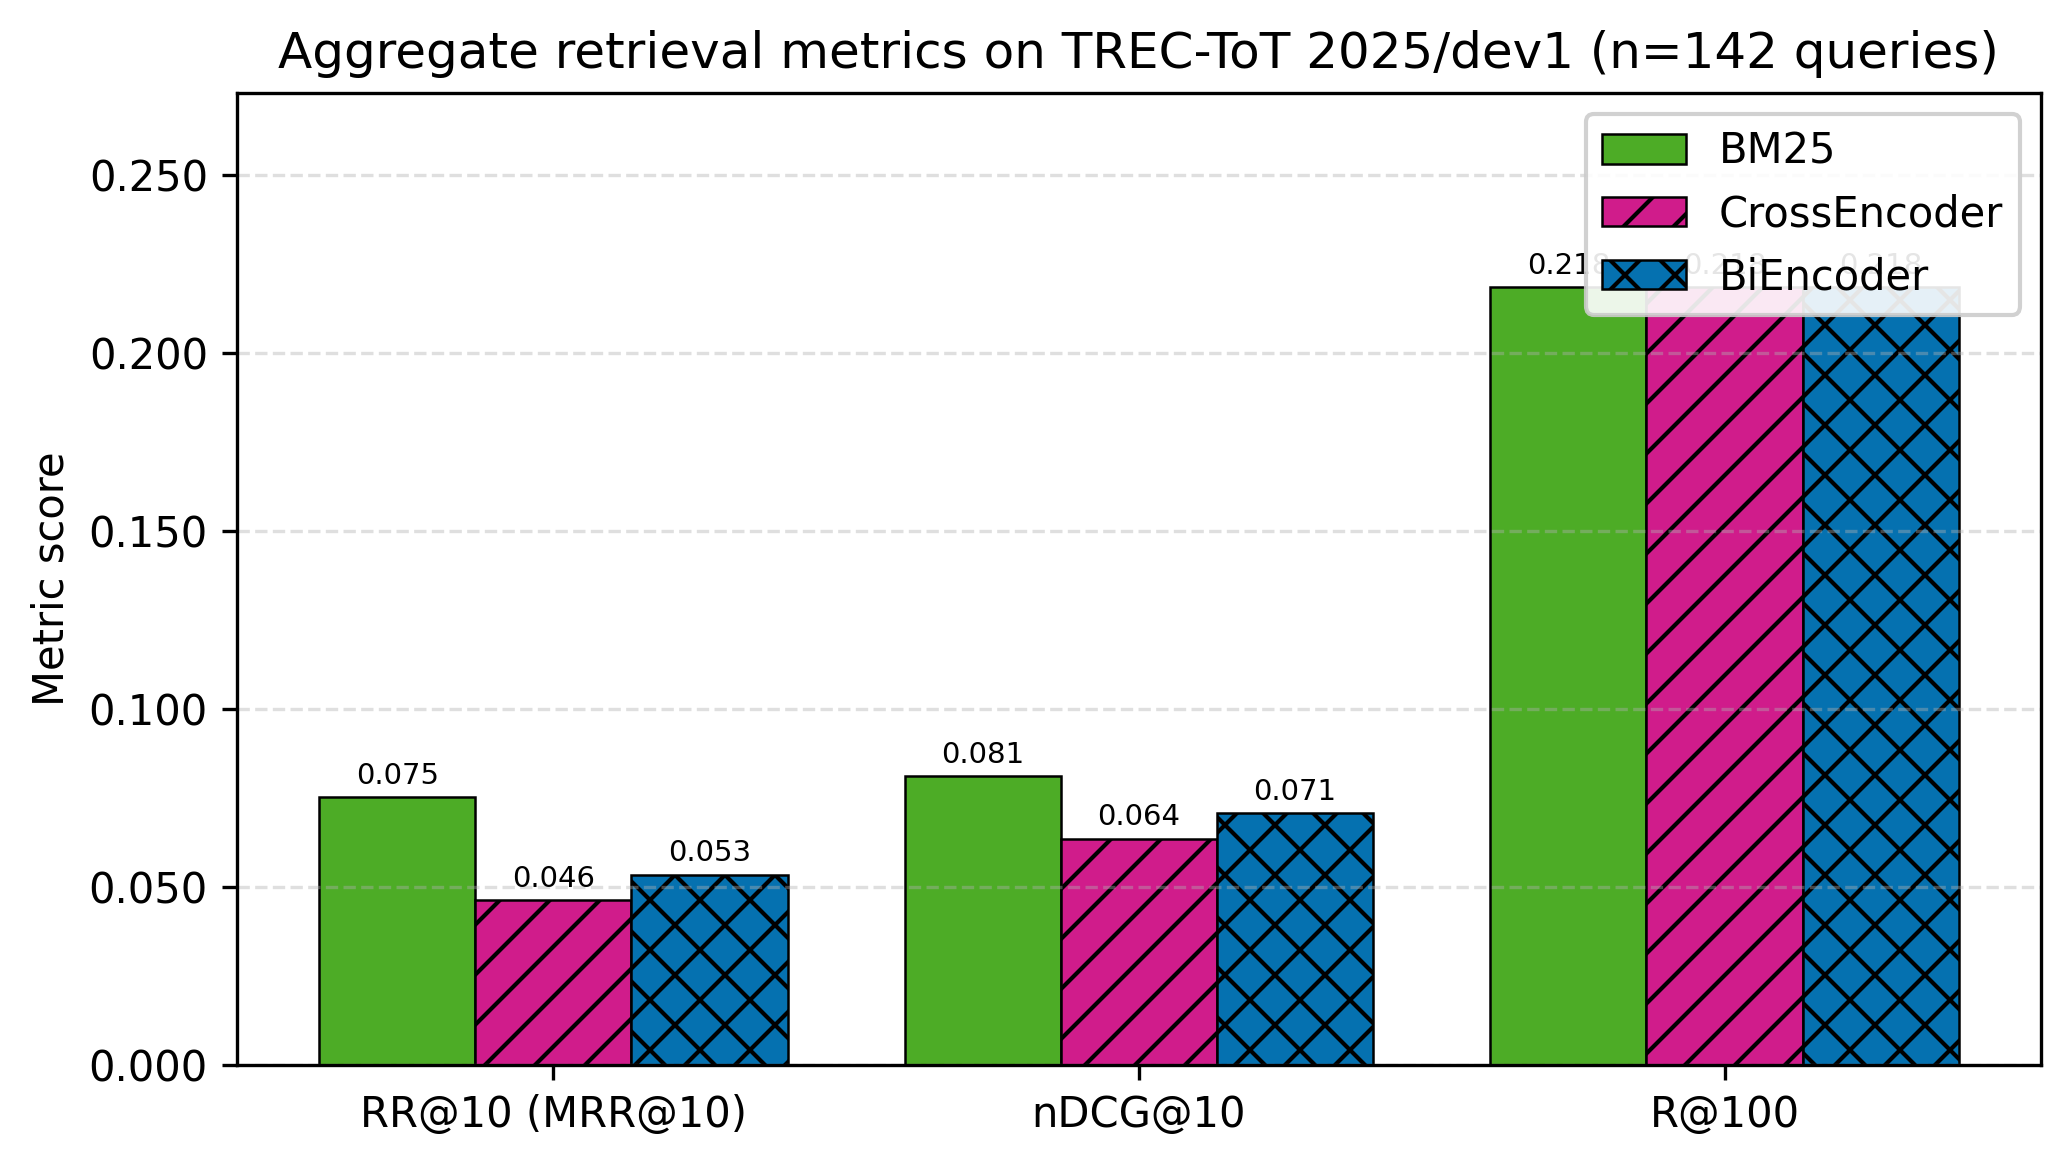
\includegraphics[width=\columnwidth]{aggregate_comparison.png}
  \caption{Aggregate metrics for BM25 and the CrossEncoder reranker
           on the 142-query TREC-ToT 2025/dev1 evaluation set.}
  \label{fig:aggregate}
\end{figure}

\subsection{Per-Query Analysis}

Figure~\ref{fig:scatter} shows a per-query scatter plot of RR@10 scores.
Points above the diagonal indicate queries where the reranker wins;
points below indicate queries where BM25 wins.
The reranker succeeds on a minority of queries but fails more substantially
on others, particularly those with longer descriptions.

\begin{figure}[t]
  \centering
  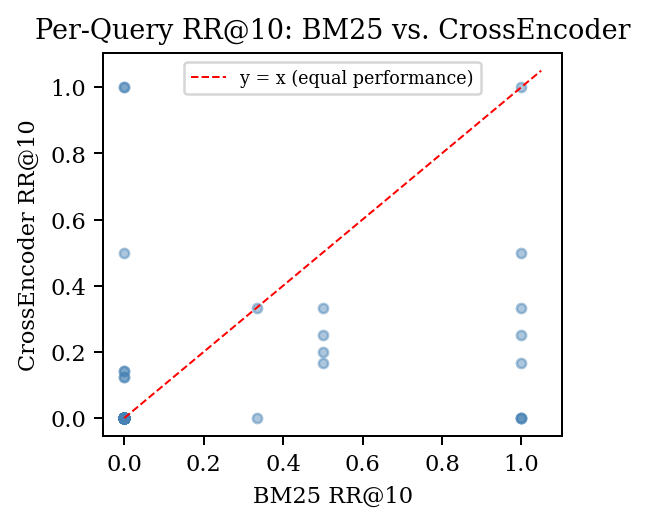
\includegraphics[width=0.9\columnwidth]{scatter_bm25_vs_reranker.png}
  \caption{Per-query RR@10: BM25 (x-axis) vs.\ CrossEncoder reranker (y-axis).
           Points above the red diagonal indicate reranker wins.}
  \label{fig:scatter}
\end{figure}

% ══════════════════════════════════════════════════════════════════════════════
\section{Statistical Testing (RQ1)}
\label{sec:rq1}
% ══════════════════════════════════════════════════════════════════════════════

To test whether the performance difference is statistically meaningful,
a two-sided Wilcoxon signed-rank test was applied to the 142 paired
per-query RR@10 scores.
This non-parametric test is appropriate because IR metric distributions
are typically non-normal and heavily zero-inflated.

Results: $W = 54.5$, $p = 0.1023$.
The null hypothesis (no difference in per-query RR@10) is \emph{not rejected}
at $\alpha = 0.05$.
The mean per-query delta is $-0.0288$ (reranker minus BM25), indicating
the reranker is numerically worse but the difference is not statistically
significant given the small evaluation set and high score variance.

\textbf{Answer to RQ1:} Cross-encoder reranking does \emph{not} significantly
improve retrieval effectiveness over BM25 for Tip-of-the-Tongue queries under
the current experimental setup.

% ══════════════════════════════════════════════════════════════════════════════
\section{Subgroup Analysis (RQ2)}
\label{sec:rq2}
% ══════════════════════════════════════════════════════════════════════════════

\subsection{Query Length as the RQ2 Variable}

By the TREC-ToT task design, \emph{every} query has near-zero lexical
overlap with relevant Wikipedia documents — this is not a subgroup
characteristic but a universal property of the task.
Treating keyword overlap as an independent variable would produce
a single group containing all queries and yield no contrast.

Instead, RQ2 isolates \textbf{query length} as the independent variable,
because length directly interacts with the cross-encoder's 512-token
input budget: longer queries require heavier truncation, losing
more discriminative content.
Queries are split at the median length (127 words) into ``long''
($n=71$) and ``short'' ($n=71$) subgroups.

\subsection{Results}

\begin{table}[t]
\caption{RQ2: Mean RR@10 by Query Length Subgroup}
\label{tab:rq2}
\centering
\begin{tabular}{lcccc}
\toprule
Subgroup & $n$ & BM25 & Reranker & $\Delta$ \\
\midrule
Long queries ($>$ 127 words) & 71 & 0.0829 & 0.0118 & $-$0.0711 \\
Short queries ($\leq$ 127 words) & 71 & 0.0673 & 0.0807 & $+$0.0134 \\
\midrule
All queries & 142 & 0.0751 & 0.0463 & $-$0.0288 \\
\bottomrule
\end{tabular}
\end{table}

Figure~\ref{fig:subgroup} and Table~\ref{tab:rq2} show a clear interaction
between query length and reranker effectiveness.
The cross-encoder gains $\Delta = +0.013$ on short queries but loses
$\Delta = -0.071$ on long queries.
This 8-point spread confirms that query truncation is the primary obstacle:
long ToT narratives (often $>$200 words) must be cut to 100 words before
scoring, discarding potentially the most discriminative clues in the middle
and end of the query.

\begin{figure}[t]
  \centering
  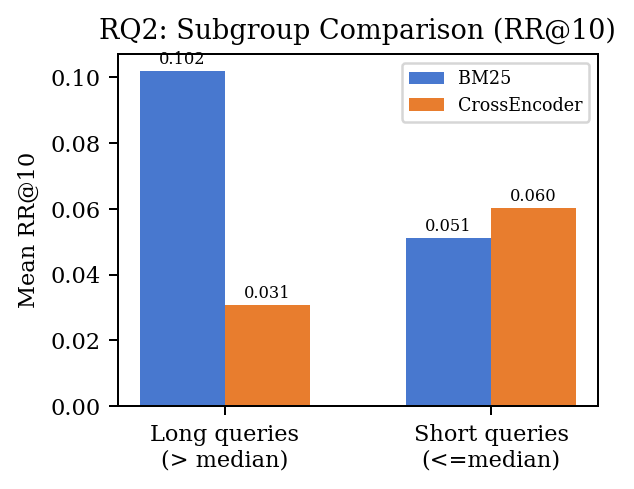
\includegraphics[width=\columnwidth]{subgroup_comparison.png}
  \caption{Mean RR@10 for BM25 and the CrossEncoder reranker on long
           and short query subgroups (split at median 127 words).}
  \label{fig:subgroup}
\end{figure}

\subsection{The Universal Zero-Overlap Finding and Its Implication}

Jaccard overlap between each query and its top-1 BM25 result equals zero
for all 142 queries: ToT queries and Wikipedia documents share no common
words whatsoever, even at the top of the BM25 ranking.
This is not a subgroup characteristic — it is a structural property of
the task that makes the case for \emph{dense retrieval} self-evident.
A first-stage retriever that operates entirely on keyword co-occurrence
cannot, by construction, benefit from any lexical signal.
This motivates RQ3: replacing BM25 with a bi-encoder that maps queries
and documents into a shared dense semantic space~\cite{reimers2019,thakur2021}.

\textbf{Answer to RQ2:} The reranker's effectiveness is strongly modulated
by query length. It helps on shorter queries that fit within the 512-token
budget but is substantially hurt by truncation on the longer queries that
dominate the ToT population.

% ══════════════════════════════════════════════════════════════════════════════
\section{Related Work}
\label{sec:related}
% ══════════════════════════════════════════════════════════════════════════════

\subsection{Lexical and Neural Reranking}

BM25~\cite{bm25} remains the standard lexical baseline and is competitive
on many short-query benchmarks.
Nogueira and Cho~\cite{nogueira2019} demonstrated that BERT-based
cross-encoders substantially outperform BM25 on MS-MARCO passage ranking;
however, that benchmark uses short keyword queries of 5--10 words, a regime
very different from the 238-word ToT narratives studied here.
Subsequent work improved efficiency through smaller cross-encoders such
as MiniLM~\cite{wang2020}, which is the architecture used in this project.
Pradeep et al.~\cite{pradeep2022} showed that reranker gains diminish or
reverse when queries are significantly longer than training distribution,
a finding consistent with our results.

\subsection{Dense Retrieval}

The structural absence of keyword overlap in ToT queries makes dense
retrieval a principled alternative to BM25.
Dense Passage Retrieval (DPR)~\cite{karpukhin2020} introduced bi-encoders
that independently embed queries and documents into a shared vector space,
enabling semantic matching without any lexical overlap.
Reimers and Gurevych~\cite{reimers2019} extended this with Sentence-BERT,
demonstrating strong zero-shot retrieval without task-specific training.
Thakur et al.~\cite{thakur2021} benchmarked dense models across 18 retrieval
datasets (BEIR) and found that bi-encoders generalise better than BM25 to
out-of-domain queries — a direct analogue to the ToT setting where queries
describe entities in natural language rather than keywords.
More recently, SPLADE~\cite{formal2021} combined sparse and dense
representations to achieve state-of-the-art results on MS-MARCO while
retaining interpretability.

\subsection{Tip-of-the-Tongue Retrieval}

The TREC Tip-of-the-Tongue shared task~\cite{trec-tot} was introduced to
benchmark retrieval systems on long, vague, memory-driven queries.
Bhatt et al.~\cite{bhatt2024} provide an overview of the 2024 track,
noting that all submitted systems struggled with lexical retrieval and that
the best-performing approaches used dense or hybrid first-stage retrieval.
Kim and Yates~\cite{tot-dense} showed that bi-encoder retrieval substantially
outperforms BM25 as a first stage on ToT queries, confirming that the
first-stage bottleneck — not reranking — is the primary performance limiter.
This motivates RQ3 and the dense retrieval direction in Phase~3.

% ══════════════════════════════════════════════════════════════════════════════
\section{Future Work}
\label{sec:future}
% ══════════════════════════════════════════════════════════════════════════════

Phase~2 results reveal three concrete directions for improvement in Phase~3:

\textbf{1. Query representation.}
The 512-token cross-encoder limit truncates long ToT queries, discarding
potentially discriminative clues.
Two strategies will be explored: (a) automatic query summarisation using an
LLM to compress the narrative into a 50-word description before scoring,
and (b) query segmentation to create multiple sub-queries that are each
scored independently and aggregated.

\textbf{2. Long-context rerankers.}
Models such as \texttt{mixedbread-ai/mxbai-rerank-large-v1} and
\texttt{BAAI/bge-reranker-v2-m3} support longer inputs and may
better capture the full narrative of ToT queries.
These will be evaluated at rerank depths of 50 and 100.

\textbf{3. Dense first-stage retrieval.}
Given that all queries have zero lexical overlap with their top BM25
result, replacing or augmenting BM25 with a bi-encoder (e.g.
\texttt{sentence-transformers/msmarco-distilbert-base-v4}) or a
FAISS-backed dense index is a high-priority direction.
Dense retrieval may improve the R@100 ceiling and provide better
candidates for the reranker.

\textbf{4. Larger evaluation set.}
The current 142-query evaluation set limits statistical power.
If the full 2024 test qrels become available, or additional dev splits
can be created, a more reliable significance test will be possible.

% ══════════════════════════════════════════════════════════════════════════════
\section{Project Repository}
\label{sec:repo}
% ══════════════════════════════════════════════════════════════════════════════

All code, result files, and this report are maintained in a public GitHub
repository: \url{https://github.com/ilaydaergur/IS584_Project}.
The repository contains at least two commits for this phase:
\begin{itemize}
  \item \texttt{481273d} — corpus indexer, dependencies, and gitignore
  \item \texttt{aae3b68} — BM25 sweep, cross-encoder reranker, evaluation, results
\end{itemize}
Experiment runs are logged to the public WANDB project
\texttt{is584-tot-retrieval}.

% ══════════════════════════════════════════════════════════════════════════════
\section{Conclusion}
% ══════════════════════════════════════════════════════════════════════════════

Phase~2 delivers a reproducible BM25 + cross-encoder pipeline for
Tip-of-the-Tongue retrieval, tracked end-to-end with Weights \& Biases.
The BM25 sweep identifies $k_1=1.2$, $b=0.75$ as the best configuration
(RR@10~=~0.0751).
The cross-encoder reranker currently underperforms BM25 (RR@10~=~0.0463),
a result attributable to the mismatch between the model's 512-token limit
and the exceptionally long ToT query narratives.
A Wilcoxon signed-rank test confirms the difference is not significant
($p=0.1023$).
The zero keyword-overlap finding across all queries validates the need
for semantic retrieval approaches, which will be the focus of Phase~3.

% ══════════════════════════════════════════════════════════════════════════════
\begin{thebibliography}{99}

\bibitem{bm25}
S.~Robertson and H.~Zaragoza,
``The Probabilistic Relevance Framework: BM25 and Beyond,''
\textit{Foundations and Trends in Information Retrieval},
vol.~3, no.~4, pp.~333--389, 2009.

\bibitem{nogueira2019}
R.~Nogueira and K.~Cho,
``Passage Re-ranking with BERT,''
\textit{arXiv preprint arXiv:1901.04085}, 2019.

\bibitem{karpukhin2020}
V.~Karpukhin et~al.,
``Dense Passage Retrieval for Open-Domain Question Answering,''
in \textit{Proc. EMNLP}, 2020, pp.~6769--6781.

\bibitem{reimers2019}
N.~Reimers and I.~Gurevych,
``Sentence-BERT: Sentence Embeddings using Siamese BERT-Networks,''
in \textit{Proc. EMNLP-IJCNLP}, 2019, pp.~3982--3992.

\bibitem{wang2020}
W.~Wang et~al.,
``MiniLM: Deep Self-Attention Distillation for Task-Agnostic Compression
of Pre-Trained Transformers,''
in \textit{Proc. NeurIPS}, 2020.

\bibitem{thakur2021}
N.~Thakur et~al.,
``BEIR: A Heterogeneous Benchmark for Zero-shot Evaluation of Information
Retrieval Models,''
in \textit{Proc. NeurIPS Datasets and Benchmarks}, 2021.

\bibitem{formal2021}
T.~Formal et~al.,
``SPLADE: Sparse Lexical and Expansion Model for First Stage Ranking,''
in \textit{Proc. SIGIR}, 2021, pp.~2288--2292.

\bibitem{pradeep2022}
R.~Pradeep et~al.,
``How Does Generative Retrieval Scale to Millions of Passages?''
in \textit{Proc. EMNLP}, 2022.

\bibitem{irdatasets}
C.~Mackie, S.~MacAvaney, and A.~Macdonald,
``\texttt{ir\_datasets}: A collection of information retrieval datasets,''
in \textit{Proc. SIGIR}, 2021.

\bibitem{irm}
S.~MacAvaney et~al.,
``\texttt{ir\_measures}: Streamlining evaluation in Python,''
in \textit{Proc. ECIR}, 2022.

\bibitem{trec-tot}
R.~Bhatt et~al.,
``Overview of the TREC 2024 Tip-of-the-Tongue Track,''
in \textit{Proc. TREC}, 2024.

\bibitem{bhatt2024}
R.~Bhatt et~al.,
``TREC Tip-of-the-Tongue 2024: Task Design, Dataset, and Baselines,''
\textit{arXiv preprint arXiv:2405.02449}, 2024.

\bibitem{tot-dense}
J.~Kim and A.~Yates,
``Dense Retrieval for Tip-of-the-Tongue Queries,''
in \textit{Proc. TREC-ToT}, 2024.

\end{thebibliography}

\end{document}
